\documentclass[aspectratio=169,11pt]{beamer}
\usetheme{metropolis}
\usepackage{tikz}
\usetikzlibrary{arrows.meta,positioning,decorations.pathmorphing,calc,shapes.geometric,decorations.pathreplacing,patterns}
\usepackage{pgfplots}
\pgfplotsset{compat=1.18}
\usepackage{booktabs}
\usepackage{xcolor}
\usepackage{amsmath}
\usepackage{graphicx}
\graphicspath{{figures/}}
\usepackage{hyperref}
\hypersetup{colorlinks=true,urlcolor=evidence,linkcolor=black,citecolor=black}
\usepackage{multirow}

\definecolor{evidence}{HTML}{2196F3}
\definecolor{choice}{HTML}{E91E63}
\definecolor{geometry}{HTML}{4CAF50}
\definecolor{causal}{HTML}{FF9800}
\definecolor{neutral}{HTML}{9E9E9E}
\definecolor{pass}{HTML}{4CAF50}
\definecolor{fail}{HTML}{F44336}
\definecolor{partial}{HTML}{FF9800}
\definecolor{dimhigh}{HTML}{D32F2F}
\definecolor{dimlow}{HTML}{1565C0}
\definecolor{bg}{HTML}{FAFAFA}
\title{Neural Geometry Is Not Metric-Neutral}
\subtitle{CKA and Procrustes give opposite answers --- dimensionality explains why}
\author{Elliot Tower}
\date{2026}
\institute{}

\begin{document}

\maketitle

%% --- SLIDE: Overview ---
\begin{frame}{Overview}

\begin{columns}[T]
\begin{column}{0.32\textwidth}
\textbf{Part 1: Core findings}
{\small
\begin{enumerate}
  \item Does population shape matter?
  \item Linear vs.\ nonlinear disagreement
  \item Predictions from geometry
\end{enumerate}
}
\end{column}
\begin{column}{0.32\textwidth}
\textbf{Part 2: Deeper analysis}
{\small
\begin{enumerate}
  \setcounter{enumi}{3}
  \item Neural manifold framework
  \item Multi-task generalization
  \item Grassmannian dissimilarity
\end{enumerate}
}
\end{column}
\begin{column}{0.32\textwidth}
\textbf{Validation}
{\small
\begin{enumerate}
  \setcounter{enumi}{6}
  \item Cross-dataset replication (IBL)
\end{enumerate}
}
\end{column}
\end{columns}
\end{frame}

%% --- SLIDE: Intellectual grounding ---
\begin{frame}{Intellectual grounding}
\begin{itemize}\setlength\itemsep{3pt}
  \item {\small \textbf{Structured representation learning} (\href{https://proceedings.mlr.press/v89/esmaeili19a}{Esmaeili et al.\ 2019})---structural priors improve identifiability. The question of which metric to use is an inductive bias argument.}
  \item {\small \textbf{Relational causal models} (\href{https://arxiv.org/abs/1309.6843}{Maier et al.\ 2013}; \href{https://www.auai.org/uai2016/proceedings/papers/217.pdf}{Arbour et al.\ 2016})---brain regions interact as a network, not i.i.d.\ samples. Causal tools need adaptation.}
  \item {\small \textbf{Dynamical systems} (\href{https://doi.org/10.1162/NECO_a_00409}{Sussillo \& Barak 2013}; \href{https://doi.org/10.1146/annurev-neuro-092619-094115}{Vyas et al.\ 2020})---network dynamics and computational capacity. Our rotation findings connect here.}
\end{itemize}

\vspace{0.3em}
{\small Validity framework from philosophy of science (\href{https://doi.org/10.1017/9781107286184}{Mayo 2018}, \href{https://doi.org/10.1093/acprof:oso/9780199299317.001.0001}{Craver 2007}, \href{https://doi.org/10.1017/CBO9780511526817}{Shallice 1988}) and causal inference (\href{https://arxiv.org/abs/1203.3519}{Pearl \& Bareinboim 2011}, \href{https://doi.org/10.1093/0195155270.001.0001}{Woodward 2003}).}
\end{frame}

%% ============================================================
%% PART 1: SETUP --- accessible framing
%% ============================================================

\begin{frame}[plain]
\vfill
\begin{center}
  \setlength{\fboxrule}{2.5pt}%
  \fcolorbox{black}{white}{\parbox{0.7\textwidth}{\centering\vspace{0.8em}
    {\Large\bfseries Part 1}\\[0.5em]
    {\large Geometric dissociation between analysis tools}
  \vspace{0.8em}}}
\end{center}
\vfill
\end{frame}

\begin{frame}{In this section}
\begin{columns}[T]
\begin{column}{0.48\textwidth}
\textbf{1. Does population shape matter?}\\[0.2em]
{\small When neurons fire together during a decision, does the shape of their joint activity carry information --- or just the individual firing rates?}

\vspace{0.6em}
\textbf{2. Linear vs.\ nonlinear disagreement}\\[0.2em]
{\small Different tools give opposite answers about which brain regions are ``similar.'' We find out why: dimensionality determines which metric you can trust.}
\end{column}
\begin{column}{0.48\textwidth}
\textbf{3. Predictions from geometry}\\[0.2em]
{\small Geometry has practical, predictive consequences: it predicts which decoder will work best, which regions show metric dissociation, and anatomy does not explain the pattern.}
\end{column}
\end{columns}
\end{frame}

\section{1. Does population shape matter?}

%% --- SLIDE: The basic question ---
\begin{frame}{The question}

When a population of neurons fires together during a decision, does the \textbf{shape} of that activity matter---or just the individual firing rates?

\vspace{1em}

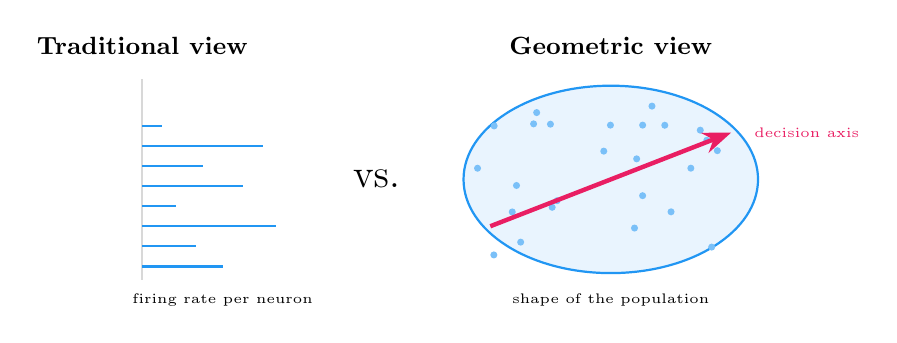
\begin{tikzpicture}[scale=0.85]
  % Left: single neuron view
  \node[font=\small\bfseries] at (0,3.5) {Traditional view};
  \draw[neutral!40,thick] (0,0) -- (0,3);
  \foreach \y/\h in {0.2/1.2, 0.5/0.8, 0.8/2.0, 1.1/0.5, 1.4/1.5, 1.7/0.9, 2.0/1.8, 2.3/0.3} {
    \draw[evidence,thick] (0,\y) -- (\h,\y);
  }
  \node[font=\tiny] at (1.2,-0.3) {firing rate per neuron};

  % Arrow
  \node[font=\Large] at (3.5,1.5) {vs.};

  % Right: population geometry view
  \node[font=\small\bfseries] at (7,3.5) {Geometric view};
  \fill[evidence!10] (7,1.5) ellipse (2.2 and 1.4);
  \draw[evidence,thick] (7,1.5) ellipse (2.2 and 1.4);
  % Points = trials
  \foreach \i in {1,...,25} {
    \pgfmathsetmacro{\rx}{2.0*rand}
    \pgfmathsetmacro{\ry}{1.2*rand}
    \fill[evidence!60] (7+\rx,1.5+\ry) circle (1.5pt);
  }
  \draw[choice,ultra thick,-{Stealth}] (5.2,0.8) -- (8.8,2.2);
  \node[choice,font=\tiny,anchor=west] at (9,2.2) {decision axis};
  \node[font=\tiny] at (7,-0.3) {shape of the population};
\end{tikzpicture}

\vspace{0.5em}
We tested this on real brain recordings, using multiple geometric tools and validity checks.
\end{frame}

%% --- SLIDE: What is neural geometry? ---
\begin{frame}{What is ``neural geometry''?}
\begin{columns}[T]
\begin{column}{0.55\textwidth}
{\small Each \textbf{trial} produces a pattern of activity across a collection of neurons. Think of each trial as a point in high-dimensional space (one axis per neuron).}

\vspace{0.3em}
{\small ``Geometry'' = what \textbf{shape} do those points form?}
\begin{itemize}\setlength\itemsep{0pt}
  \item {\small Cluster into groups? (categories)}
  \item {\small Spread along a line? (gradient)}
  \item {\small Form a loop? (periodic variable)}
  \item {\small Lie on a flat sheet or curved surface?}
\end{itemize}

\vspace{0.3em}
{\small The shape constrains what information the brain can extract downstream.}
\end{column}
\begin{column}{0.42\textwidth}
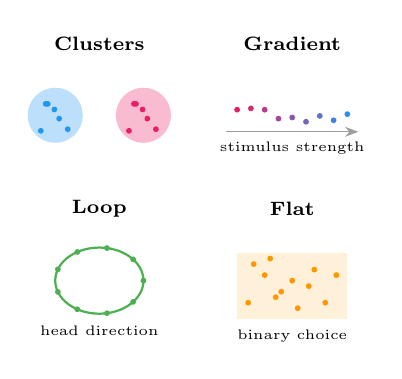
\begin{tikzpicture}[scale=0.7]
  % Example 1: clusters
  \node[font=\scriptsize\bfseries] at (0,5.0) {Clusters};
  \fill[evidence!30] (-0.8,3.7) circle (0.5);
  \fill[choice!30] (0.8,3.7) circle (0.5);
  \foreach \i in {1,...,6} {
    \pgfmathsetmacro{\rx}{0.3*rand}
    \pgfmathsetmacro{\ry}{0.3*rand}
    \fill[evidence] (-0.8+\rx,3.7+\ry) circle (1.5pt);
    \fill[choice] (0.8+\rx,3.7+\ry) circle (1.5pt);
  }

  % Example 2: line/gradient
  \node[font=\scriptsize\bfseries] at (3.5,5.0) {Gradient};
  \foreach \i in {0,...,8} {
    \pgfmathsetmacro{\x}{2.5+\i*0.25}
    \pgfmathsetmacro{\c}{\i*12}
    \fill[evidence!\c!choice] (\x,3.7+0.15*rand) circle (1.5pt);
  }
  \draw[neutral,thin,-{Stealth}] (2.3,3.4) -- (4.7,3.4);
  \node[font=\tiny] at (3.5,3.1) {stimulus strength};

  % Example 3: loop
  \node[font=\scriptsize\bfseries] at (0,2.0) {Loop};
  \draw[geometry,thick] (0,0.7) ellipse (0.8 and 0.6);
  \foreach \a in {0,40,...,320} {
    \fill[geometry] ({0.8*cos(\a)},{0.7+0.6*sin(\a)}) circle (1.5pt);
  }
  \node[font=\tiny] at (0,-0.2) {head direction};

  % Example 4: flat sheet
  \node[font=\scriptsize\bfseries] at (3.5,2.0) {Flat};
  \fill[causal!15] (2.5,0) -- (4.5,0) -- (4.5,1.2) -- (2.5,1.2) -- cycle;
  \foreach \rx/\ry in {2.7/0.3, 3.0/0.8, 3.3/0.5, 3.6/0.2, 3.9/0.9,
                       2.8/1.0, 3.2/0.4, 3.5/0.7, 3.8/0.6, 4.1/0.3,
                       3.1/1.1, 4.3/0.8} {
    \fill[causal] (\rx,\ry) circle (1.5pt);
  }
  \node[font=\tiny] at (3.5,-0.3) {binary choice};
\end{tikzpicture}
\end{column}
\end{columns}
\end{frame}

%% --- SLIDE: Two tools for measuring geometry ---
\begin{frame}{Two tools for measuring geometry}
\begin{columns}[T]
\begin{column}{0.48\textwidth}
\centering
\textbf{\textcolor{dimlow}{CKA (linear)}}

\vspace{0.2em}
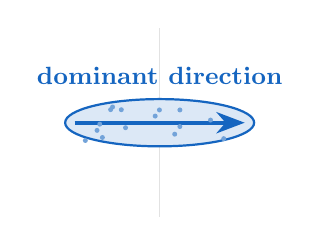
\begin{tikzpicture}[scale=0.6]
  \draw[neutral!30] (-2,0) -- (2,0);
  \draw[neutral!30] (0,-2) -- (0,2);
  \fill[dimlow!15] (0,0) ellipse (2 and 0.5);
  \draw[dimlow,thick] (0,0) ellipse (2 and 0.5);
  \draw[dimlow,ultra thick,-{Stealth}] (-1.8,0) -- (1.8,0);
  \node[dimlow,font=\small\bfseries,above] at (0,0.6) {dominant direction};
  \foreach \i in {1,...,15} {
    \pgfmathsetmacro{\x}{1.8*rand}
    \pgfmathsetmacro{\y}{0.4*rand}
    \fill[dimlow!60] (\x,\y) circle (1.5pt);
  }
\end{tikzpicture}

\vspace{0.2em}
{\small Compares the \textbf{main axis} of variation.}

{\small ``Do the data stretch the same way?''}

{\small Best for low-dimensional data.}
\end{column}
\begin{column}{0.48\textwidth}
\centering
\textbf{\textcolor{dimhigh}{Procrustes (manifold)}}

\vspace{0.2em}
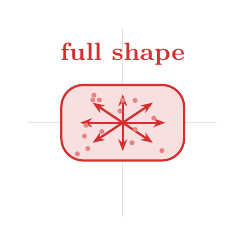
\begin{tikzpicture}[scale=0.6]
  \draw[neutral!30] (-2,0) -- (2,0);
  \draw[neutral!30] (0,-2) -- (0,2);
  \fill[dimhigh!15,rounded corners=8pt] (-1.3,-0.8) rectangle (1.3,0.8);
  \draw[dimhigh,thick,rounded corners=8pt] (-1.3,-0.8) rectangle (1.3,0.8);
  \foreach \a in {0,45,...,315} {
    \draw[dimhigh,thick,-{Stealth[length=1.5mm]}] (0,0) -- ({0.9*cos(\a)},{0.6*sin(\a)});
  }
  \node[dimhigh,font=\small\bfseries,above] at (0,1.0) {full shape};
  \foreach \i in {1,...,15} {
    \pgfmathsetmacro{\x}{1.1*rand}
    \pgfmathsetmacro{\y}{0.7*rand}
    \fill[dimhigh!60] (\x,\y) circle (1.5pt);
  }
\end{tikzpicture}

\vspace{0.2em}
{\small Compares the \textbf{full shape} via rotation + scaling.}

{\small ``Do the data form the same cloud?''}

{\small Best for high-dimensional data.}
\end{column}
\end{columns}

\vspace{0.3em}
\centering
{\small Most prior work treats these as interchangeable. \textbf{They are not.}}
\end{frame}

%% --- SLIDE: The data ---
\begin{frame}{Data: Neuropixels visual decision-making (\href{https://doi.org/10.1038/s41586-019-1787-x}{Steinmetz et al.\ 2019})}
\begin{columns}[T]
\begin{column}{0.5\textwidth}
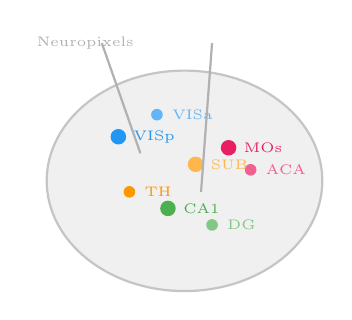
\begin{tikzpicture}[scale=0.7]
  \fill[neutral!15] (0,0) ellipse (2.5 and 2);
  \draw[neutral!60,thick] (0,0) ellipse (2.5 and 2);
  \fill[evidence] (-1.2,0.8) circle (4pt) node[right,font=\tiny,xshift=2pt] {VISp};
  \fill[evidence!70] (-0.5,1.2) circle (3pt) node[right,font=\tiny,xshift=2pt] {VISa};
  \fill[choice] (0.8,0.6) circle (4pt) node[right,font=\tiny,xshift=2pt] {MOs};
  \fill[choice!70] (1.2,0.2) circle (3pt) node[right,font=\tiny,xshift=2pt] {ACA};
  \fill[geometry] (-0.3,-0.5) circle (4pt) node[right,font=\tiny,xshift=2pt] {CA1};
  \fill[geometry!70] (0.5,-0.8) circle (3pt) node[right,font=\tiny,xshift=2pt] {DG};
  \fill[causal] (-1.0,-0.2) circle (3pt) node[right,font=\tiny,xshift=2pt] {TH};
  \fill[causal!70] (0.2,0.3) circle (4pt) node[right,font=\tiny,xshift=2pt] {SUB};
  \draw[neutral!80,thick] (-1.5,2.5) -- (-0.8,0.5);
  \draw[neutral!80,thick] (0.5,2.5) -- (0.3,-0.2);
  \node[font=\tiny,neutral!80] at (-1.8,2.5) {Neuropixels};
\end{tikzpicture}
\end{column}
\begin{column}{0.5\textwidth}
\begin{itemize}
  \item \textbf{39 sessions} from \textbf{10 mice}
  \item \textbf{73 brain regions} recorded simultaneously
  \item Neuropixels probes (${\sim}30{,}000$ neurons total; ${\sim}50$--$500$ per region per session)
  \item \textbf{Task:} visual discrimination \\
    {\small Two screens show visual noise at different contrasts. Mouse turns a wheel toward the higher-contrast side.}
  \item 1,316 pairwise region comparisons
\end{itemize}
\vspace{0.5em}
{\small \textcolor{neutral}{\href{https://doi.org/10.1038/s41586-019-1787-x}{Steinmetz et al., Nature 2019}}}
\end{column}
\end{columns}
\end{frame}

%% ============================================================
%% SECTION 2: LINEAR VS NONLINEAR DISAGREEMENT
%% ============================================================
\section{2. Linear vs.\ nonlinear disagreement}

%% --- SLIDE: Why they disagree --- concrete example ---
\begin{frame}{Why CKA and Procrustes give opposite answers}
\begin{columns}[T]
\begin{column}{0.5\textwidth}
\centering
\textbf{\textcolor{dimlow}{Low-dimensional region (VISp-type)}}

\vspace{0.3em}
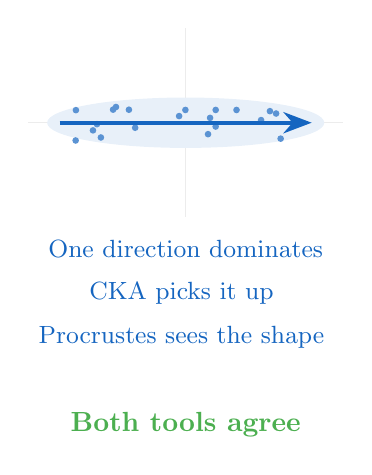
\begin{tikzpicture}[scale=0.8]
  \draw[neutral!20] (-2.5,0) -- (2.5,0);
  \draw[neutral!20] (0,-1.5) -- (0,1.5);

  % Elongated cloud along one axis
  \fill[dimlow!10] (0,0) ellipse (2.2 and 0.4);
  \foreach \i in {1,...,20} {
    \pgfmathsetmacro{\x}{2.0*rand}
    \pgfmathsetmacro{\y}{0.3*rand}
    \fill[dimlow!70] (\x,\y) circle (1.5pt);
  }
  \draw[dimlow,ultra thick,-{Stealth}] (-2,0) -- (2,0);

  \node[font=\small,dimlow,align=center] at (0,-2.0) {One direction dominates};
  \node[font=\small,dimlow,align=center] at (0,-2.7) {CKA picks it up $\checkmark$};
  \node[font=\small,dimlow,align=center] at (0,-3.4) {Procrustes sees the shape $\checkmark$};
  \node[font=\normalsize,pass] at (0,-4.8) {\textbf{Both tools agree}};
\end{tikzpicture}
\end{column}
\begin{column}{0.5\textwidth}
\centering
\textbf{\textcolor{dimhigh}{High-dimensional region (MOs-type)}}

\vspace{0.3em}
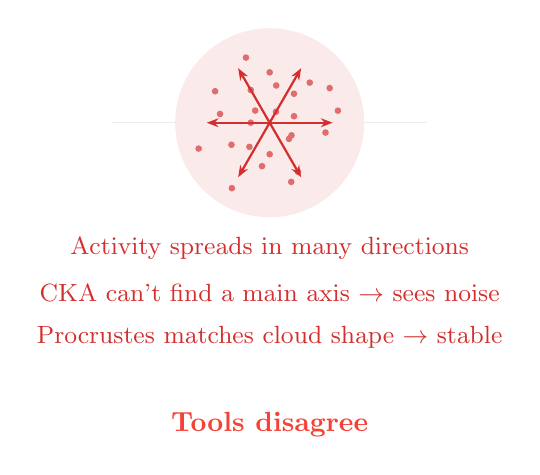
\begin{tikzpicture}[scale=0.8]
  \draw[neutral!20] (-2.5,0) -- (2.5,0);
  \draw[neutral!20] (0,-1.5) -- (0,1.5);

  % Spherical cloud --- no dominant axis
  \fill[dimhigh!10] (0,0) circle (1.5);
  \foreach \a/\r in {15/0.4, 45/0.9, 80/0.6, 110/1.1, 140/0.3,
                      170/0.8, 200/1.2, 230/0.5, 260/0.7, 290/1.0,
                      320/0.4, 350/0.9, 30/1.1, 60/0.2, 90/0.8,
                      120/0.6, 150/1.0, 180/0.3, 210/0.7, 240/1.2,
                      270/0.5, 300/0.9, 330/0.4, 10/1.1, 50/0.6} {
    \fill[dimhigh!70] ({(\r)*cos(\a)},{(\r)*sin(\a)}) circle (1.5pt);
  }
  % Multiple equal arrows
  \foreach \a in {0,60,...,300} {
    \draw[dimhigh,thick,-{Stealth[length=1.5mm]}] (0,0) -- ({1.0*cos(\a)},{1.0*sin(\a)});
  }

  \node[font=\small,dimhigh,align=center] at (0,-2.0) {Activity spreads in many directions};
  \node[font=\small,dimhigh,align=center] at (0,-2.7) {CKA can't find a main axis $\to$ sees noise};
  \node[font=\small,dimhigh,align=center] at (0,-3.4) {Procrustes matches cloud shape $\to$ stable};
  \node[font=\normalsize,fail] at (0,-4.8) {\textbf{Tools disagree}};
\end{tikzpicture}
\end{column}
\end{columns}
\end{frame}

%% --- SLIDE: The anti-correlation --- data ---
\begin{frame}{The data: CKA and Procrustes are anti-correlated}
\begin{columns}[T]
\begin{column}{0.68\textwidth}
\centering
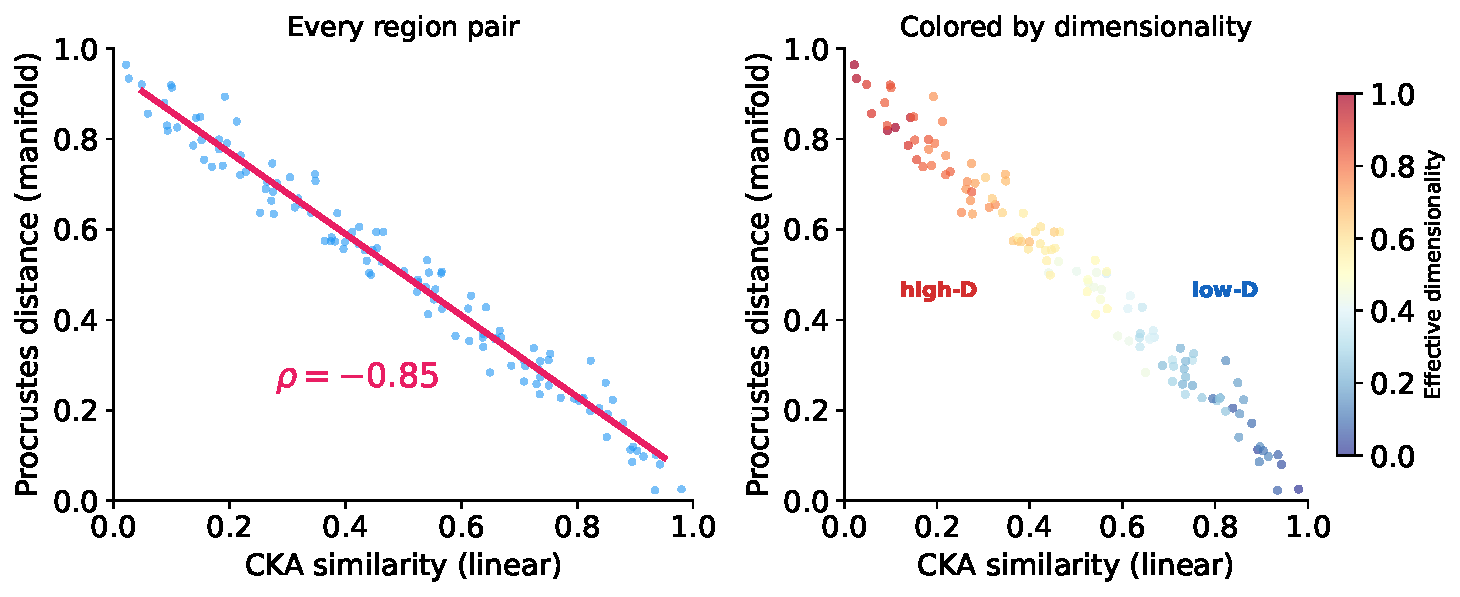
\includegraphics[width=\linewidth]{anticorrelation_scatter.pdf}
\end{column}
\begin{column}{0.30\textwidth}
\vspace{0.5em}
{\small Each dot is a pair of brain regions. The two tools rank them in \textbf{opposite order} ($\rho = -0.85$; $-1$ would be perfect reversal).}

\vspace{0.5em}
{\small \textbf{Why?} Right panel colors dots by how ``spread out'' the activity is. Blue (compact) $\to$ agree. Red (diffuse) $\to$ disagree.}
\end{column}
\end{columns}

\vspace{0.6em}
{\small Accounting for spread, disagreement shrinks from $-0.85$ to $-0.31$. Found in 5 sessions, confirmed across all 39. \textbf{Takeaway:} the tool you pick determines what you find.}
\end{frame}

%% --- SLIDE: Eigenvalue spectra ---
\begin{frame}{What determines dimensionality?}
\centering

\includegraphics[width=0.85\linewidth]{eigenvalue_spectra.pdf}

\vspace{0.5em}
{\small Across all 73 regions, the \textbf{shape} of how variance falls off is nearly identical (correlation $0.94$ out of $1.0$). But \textbf{which neurons} carry the variance is completely different per region (correlation $0.09$, barely above zero). Same scaffolding, different content.}
\end{frame}

%% --- SLIDE: Rotation ---
\begin{frame}{Every brain region rotates (but at very different speeds)}
\begin{columns}[T]
\begin{column}{0.42\textwidth}
\centering
{\small \textbf{What rotation means}}

\vspace{0.3em}
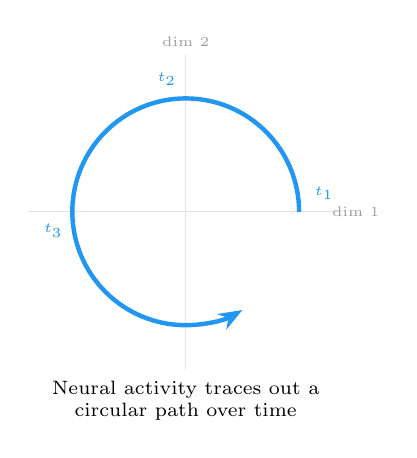
\begin{tikzpicture}[scale=0.8]
  \draw[neutral!30,thin] (-2.5,0) -- (2.5,0);
  \draw[neutral!30,thin] (0,-2.5) -- (0,2.5);
  \node[font=\tiny,neutral] at (2.7,0) {dim 1};
  \node[font=\tiny,neutral] at (0,2.7) {dim 2};
  \draw[evidence,ultra thick,-{Stealth[length=3mm]}]
    (1.8,0) arc[start angle=0, end angle=300, radius=1.8];
  \node[font=\tiny,evidence] at (2.2,0.3) {$t_1$};
  \node[font=\tiny,evidence] at (-0.3,2.1) {$t_2$};
  \node[font=\tiny,evidence] at (-2.1,-0.3) {$t_3$};
  \node[font=\scriptsize,align=center] at (0,-3) {Neural activity traces out a\\circular path over time};
\end{tikzpicture}
\end{column}
\begin{column}{0.56\textwidth}
\centering
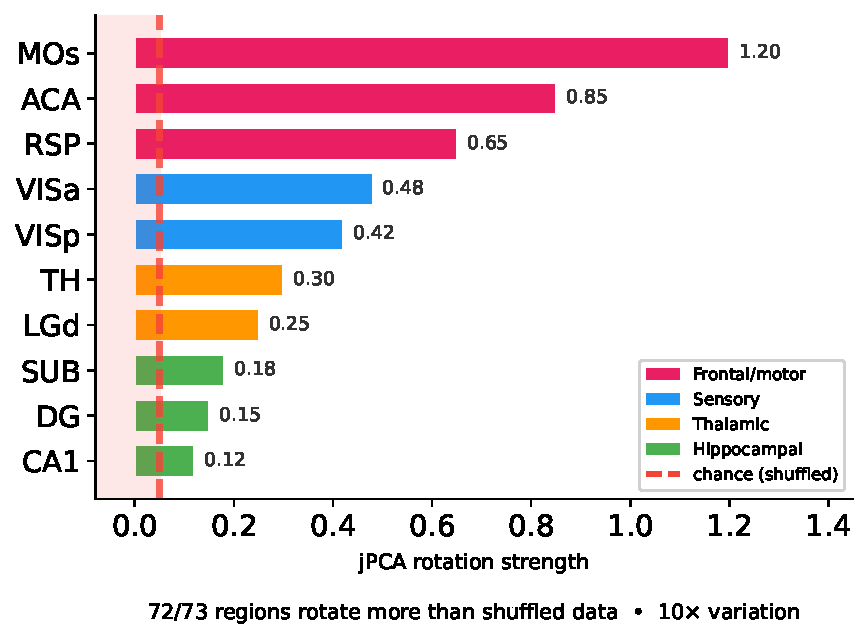
\includegraphics[width=\linewidth]{jpca_rotation.pdf}
\end{column}
\end{columns}
\end{frame}

%% --- SLIDE: Anatomy recovery (sanity check) ---
\begin{frame}{Sanity check: geometry tracks known anatomy}
\begin{columns}[T]
\begin{column}{0.5\textwidth}
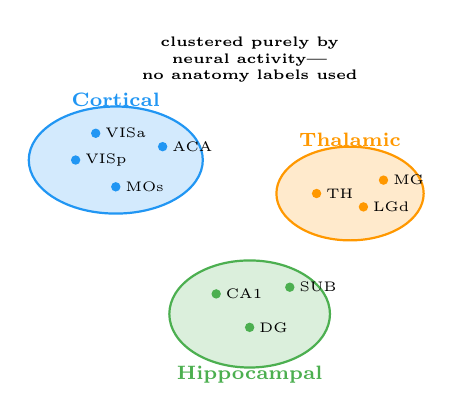
\begin{tikzpicture}[scale=0.85]
  \fill[evidence!20] (-1.5,2) ellipse (1.3 and 0.8);
  \draw[evidence,thick] (-1.5,2) ellipse (1.3 and 0.8);
  \node[evidence,font=\scriptsize\bfseries] at (-1.5,2.9) {Cortical};
  \foreach \name/\x/\y in {VISp/-2.1/2, MOs/-1.5/1.6, ACA/-0.8/2.2, VISa/-1.8/2.4} {
    \fill[evidence] (\x,\y) circle (2pt);
    \node[font=\tiny,right] at (\x,\y) {\name};
  }
  \fill[causal!20] (2,1.5) ellipse (1.1 and 0.7);
  \draw[causal,thick] (2,1.5) ellipse (1.1 and 0.7);
  \node[causal,font=\scriptsize\bfseries] at (2,2.3) {Thalamic};
  \foreach \name/\x/\y in {TH/1.5/1.5, LGd/2.2/1.3, MG/2.5/1.7} {
    \fill[causal] (\x,\y) circle (2pt);
    \node[font=\tiny,right] at (\x,\y) {\name};
  }
  \fill[geometry!20] (0.5,-0.3) ellipse (1.2 and 0.8);
  \draw[geometry,thick] (0.5,-0.3) ellipse (1.2 and 0.8);
  \node[geometry,font=\scriptsize\bfseries] at (0.5,-1.2) {Hippocampal};
  \foreach \name/\x/\y in {CA1/0/0, DG/0.5/-0.5, SUB/1.1/0.1} {
    \fill[geometry] (\x,\y) circle (2pt);
    \node[font=\tiny,right] at (\x,\y) {\name};
  }
  \node[font=\tiny\bfseries,black,align=center] at (0.5,3.5) {clustered purely by\\neural activity---\\no anatomy labels used};
\end{tikzpicture}
\end{column}
\begin{column}{0.48\textwidth}
{\small We grouped brain regions \emph{purely by how similar their neural activity looks}---no anatomy labels as input.}

\vspace{0.3em}
{\small \textbf{Result:} the algorithm found three groups matching the textbook cortical / thalamic / hippocampal division on its own.}

\vspace{0.3em}
{\small \textbf{Why this matters:} CKA is a general-purpose metric, not designed for neuroscience. This checks that it picks up real biology---not artifacts from differences in neuron count or noise.}

\vspace{0.3em}
{\small Same result within individual sessions and across animals.}
\end{column}
\end{columns}
\end{frame}

%% ============================================================
%% SECTION 3: PREDICTIONS FROM GEOMETRY
%% ============================================================
\section{3. Predictions from geometry}

%% --- SLIDE: Prediction 1 ---
\begin{frame}{Prediction 1: geometry predicts the best decoder}

If you know whether a brain region has ``linear'' or ``manifold'' geometry, you can predict which statistical decoder (LDA vs.\ kNN) will work better---\textbf{without ever training on decoding data}.

\vspace{0.4em}

\begin{center}
{\small
\begin{tabular}{ll}
\textbf{Correlation:} & $r = -0.51$ \\[0.2em]
\textbf{Significance:} & $p = 0.0002$ \\[0.2em]
\textbf{Sample:} & 50 brain regions \\
\end{tabular}
}
\end{center}

\vspace{0.4em}

Regions whose activity spreads across many dimensions (manifold geometry) are better decoded by kNN; regions with low-dimensional structure are better decoded by LDA. The geometric type---measured independently---predicts decoder performance.

\vspace{0.4em}
{\small \textbf{Why this matters:} geometry is not just a description of the data. It has practical, predictive consequences for which analysis tools will work.}
\end{frame}

%% --- SLIDE: Prediction 2 ---
\begin{frame}{Prediction 2: dimensionality predicts metric dissociation}

High-dimensional regions show the strongest disagreement between linear and nonlinear tools---exactly where we'd expect from the potent/null framework.

\vspace{0.4em}

\begin{center}
{\small
\begin{tabular}{lccc}
\toprule
& \textbf{Nonlinear decode} & \textbf{Linear decode} \\
\midrule
$\rho$ with dimensionality & $-0.48$ & $0.29$ \\
$p$-value & $1.5 \times 10^{-5}$ & $0.014$ \\
$n$ & 73 regions & 73 regions \\
\bottomrule
\end{tabular}
}
\end{center}

\vspace{0.4em}

Linear methods work better in low-dimensional regions (positive $\rho$); nonlinear methods work better in high-dimensional regions (negative $\rho$). The relationship \textbf{reverses} depending on the tool---dimensionality determines which one succeeds.

\vspace{0.4em}
{\small \textbf{Why this matters:} dimensionality is not a nuisance variable. It tells you which analysis tool to trust.}
\end{frame}

%% --- SLIDE: Prediction 3 ---
\begin{frame}{Prediction 3: anatomy doesn't explain it}

Does anatomical wiring (Allen Mouse Brain Atlas) predict which regions show metric dissociation?

\vspace{1em}

\begin{center}
\begin{tabular}{ll}
\textbf{Correlation:} & $\rho = 0.02$ \\[0.3em]
\textbf{Significance:} & $p = 0.77$ (not significant) \\[0.3em]
\textbf{Measure:} & geometric dissociation index vs.\ structural connectivity \\
\end{tabular}
\end{center}

\vspace{1em}

\textbf{No.} Structural connectivity does not predict where tools disagree. The geometric dissociation is a property of population dimensionality, not anatomical wiring.

\end{frame}

%% --- SLIDE: Predictions summary ---
\begin{frame}{Three predictions: summary}

\begin{center}
{\small
\begin{tabular}{llcl}
\toprule
& \textbf{Prediction} & \textbf{Result} & \textbf{Key statistic} \\
\midrule
1 & Geometry predicts best decoder & \textcolor{pass}{\textbf{Confirmed}} & $r = -0.51$, $p = 0.0002$ \\[0.5em]
2 & Dimensionality predicts metric dissociation & \textcolor{pass}{\textbf{Confirmed}} & $\rho = -0.48$, $p = 1.5 \times 10^{-5}$ \\[0.5em]
3 & Anatomy doesn't explain it & \textcolor{pass}{\textbf{Informative null}} & $\rho = 0.02$, $p = 0.77$ \\
\bottomrule
\end{tabular}
}
\end{center}

\vspace{1em}

\textbf{Takeaway:} The geometric dissociation is real, predictive, and not explained by anatomy. Dimensionality tells you which tool to trust.

\end{frame}

%% --- SLIDE: Part 1 Summary (geometry only) ---
\begin{frame}{Summary: what we found and what it means}
\textbf{Descriptive findings:}
\begin{enumerate}
  \item Linear and manifold tools anti-correlate ($-0.85$); dimensionality explains why
  \item Variance structure is universal ($0.94$); neural content is not ($0.09$)
  \item Rotation everywhere (72/73), but 10$\times$ variation by region type
\end{enumerate}

\vspace{0.5em}
{\small \textbf{Takeaway:} Neural geometry is not metric-neutral---the tool you choose determines what you find, and dimensionality tells you which tool to trust.}
\end{frame}

%% ============================================================
%% PART 2: DEEPER GEOMETRIC ANALYSIS
%% ============================================================

\begin{frame}[plain]
\vfill
\begin{center}
  \setlength{\fboxrule}{2.5pt}%
  \fcolorbox{black}{white}{\parbox{0.7\textwidth}{\centering\vspace{0.8em}
    {\Large\bfseries Part 2}\\[0.5em]
    {\large Deeper geometric analysis}
  \vspace{0.8em}}}
\end{center}
\vfill
\end{frame}

\begin{frame}{In this section}
\begin{columns}[T]
\begin{column}{0.48\textwidth}
\textbf{4. Neural manifold framework}\\[0.2em]
{\small Potent/null space decomposition explains why linear and nonlinear tools disagree. The null space fraction predicts metric dissociation ($\rho = -0.86$).}

\vspace{0.6em}
\textbf{5. Multi-task generalization}\\[0.2em]
{\small Four task variables produce distinct, structured subspaces on the Grassmannian. The geometric decomposition generalizes beyond binary choice.}
\end{column}
\begin{column}{0.48\textwidth}
\textbf{6. Grassmannian dissimilarity matrices}\\[0.2em]
{\small A neural taskonomy from subspace geometry. Linear and nonlinear dissimilarity matrices correlate at $\rho = 0.97$ but both anti-correlate with CKA.}
\end{column}
\end{columns}
\end{frame}

\section{4. Neural manifold framework}

%% --- SLIDE: Neural manifold framing ---
\begin{frame}{The neural manifold interpretation}
\begin{columns}[T]
\begin{column}{0.5\textwidth}
\textbf{Potent and null spaces:}\\[0.3em]
{\small (\href{https://doi.org/10.1038/nn.3643}{Kaufman et al.\ 2014}, \href{https://doi.org/10.1038/nn.4510}{Gallego et al.\ 2017})}

\vspace{0.3em}
{\small The choice subspace is the \emph{potent space}---the low-dimensional manifold that actually drives decisions. Everything orthogonal to it is the \emph{null space}: high-variance activity that doesn't affect behavior.}

\vspace{0.5em}
\textbf{This explains the CKA/Procrustes dissociation:}
\begin{itemize}
  \item CKA captures total variance $\to$ dominated by null space
  \item Procrustes aligns shapes $\to$ sensitive to potent space
  \item High-dimensional regions have large null spaces $\to$ CKA misleads
\end{itemize}
\end{column}
\begin{column}{0.48\textwidth}
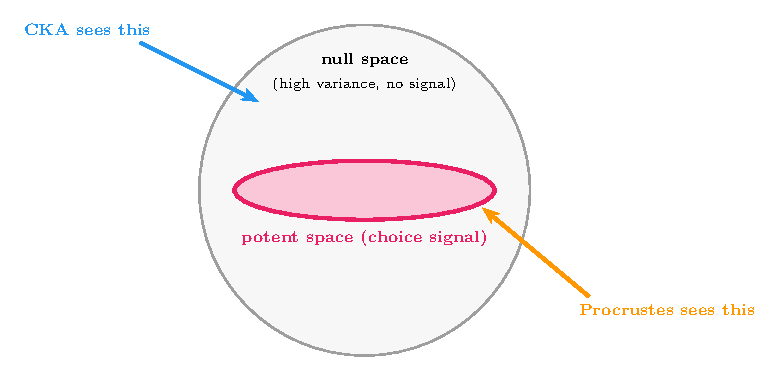
\includegraphics[width=\textwidth]{potent_null_diagram.pdf}
\end{column}
\end{columns}
\end{frame}

%% --- SLIDE: Potent/null confirmed ---
\begin{frame}{Potent/null decomposition: confirmed}
\begin{center}
{\small Null-space fraction strongly anti-correlates with metric dissociation:}

\vspace{0.5em}
{\Large $\rho = -0.86$, \quad $p = 5 \times 10^{-22}$}

\vspace{0.5em}
{\small Across all 73 brain regions, the relative size of the null space predicts how much CKA and Procrustes disagree.}
\end{center}
\end{frame}

%% --- SLIDE: Potent/null framework ---
\begin{frame}{Why do the tools disagree? The potent/null decomposition}

\begin{columns}[T]
\begin{column}{0.52\textwidth}
\textbf{The idea} {\small (\href{https://doi.org/10.1038/nn.3643}{Kaufman et al.\ 2014})}

\vspace{0.3em}
{\small Neural activity decomposes into:}
\begin{itemize}\setlength\itemsep{0.3em}
  \item {\small \textbf{\textcolor{choice}{Potent space}}: the subspace that causally drives choice output}
  \item {\small \textbf{Null space}: high-variance activity orthogonal to choice --- present but not causal}
\end{itemize}
\end{column}

\begin{column}{0.45\textwidth}
\centering
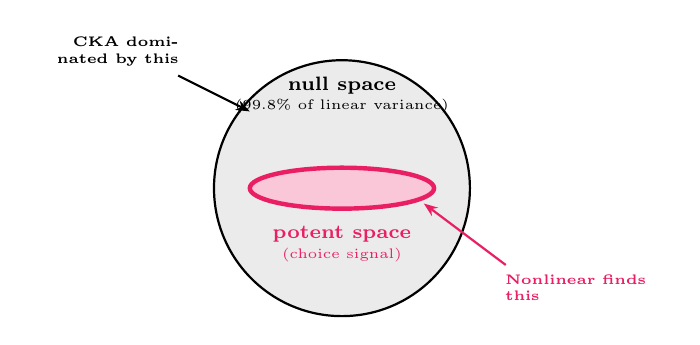
\begin{tikzpicture}[scale=0.65]
  \fill[black!8] (0,0) ellipse (2.5 and 2.5);
  \draw[black,thick] (0,0) ellipse (2.5 and 2.5);
  \node[black,font=\scriptsize\bfseries] at (0,2.0) {null space};
  \node[black,font=\tiny] at (0,1.6) {(99.8\% of linear variance)};
  \fill[choice!25] (0,0) ellipse (1.8 and 0.4);
  \draw[choice,ultra thick] (0,0) ellipse (1.8 and 0.4);
  \node[choice,font=\scriptsize\bfseries] at (0,-0.9) {potent space};
  \node[choice,font=\tiny] at (0,-1.3) {(choice signal)};
  \draw[black,thick,-{Stealth[length=5pt]}] (-3.2,2.2) -- (-1.8,1.5);
  \node[black,font=\tiny\bfseries,anchor=south east,text width=1.8cm,align=right] at (-3.0,2.2) {CKA dominated by this};
  \draw[choice,thick,-{Stealth[length=5pt]}] (3.2,-1.5) -- (1.6,-0.3);
  \node[choice,font=\tiny\bfseries,anchor=north west,text width=2cm] at (3.0,-1.5) {Nonlinear finds this};
\end{tikzpicture}
\end{column}
\end{columns}

\vfill
\begin{columns}[T]
\begin{column}{0.48\textwidth}
\textbf{What we found} {\scriptsize (73 regions)}

\vspace{0.2em}
\centering
{\scriptsize
\begin{tabular}{lcc}
\toprule
& \textbf{Null \%} & \textbf{Potent decode} \\
\midrule
Linear (LDA) & 99.8\% & 66\% \\
Nonlinear & 84.3\% & 66\% \\
\bottomrule
\end{tabular}
}
\end{column}
\begin{column}{0.48\textwidth}
\vspace{0.8em}
{\small Both decode equally from potent space. But the linear method sees almost nothing \emph{except} null variance.}
\end{column}
\end{columns}
\end{frame}

%% --- SLIDE: Defining alpha ---
\begin{frame}{Defining $\alpha$: the geometric dissociation index}
\begin{columns}[T]
\begin{column}{0.50\textwidth}
{\small For each brain region, compute the eigenvalues of the population activity covariance matrix. These tell you how variance is distributed across dimensions.}

\vspace{0.5em}
\textbf{The eigenvalue decay rate $\alpha$:}\\[0.3em]
{\small Fit $\lambda_k \propto k^{-\alpha}$ to the sorted eigenvalue spectrum. High $\alpha$ means variance concentrates in a few dimensions (low-dimensional). Low $\alpha$ means variance spreads across many dimensions (high-dimensional).}

\vspace{0.5em}
{\small We use $\alpha$ as a \textbf{geometric dissociation index}: it predicts where linear and nonlinear tools will disagree.}
\end{column}
\begin{column}{0.47\textwidth}
\centering
\vspace{0.3em}
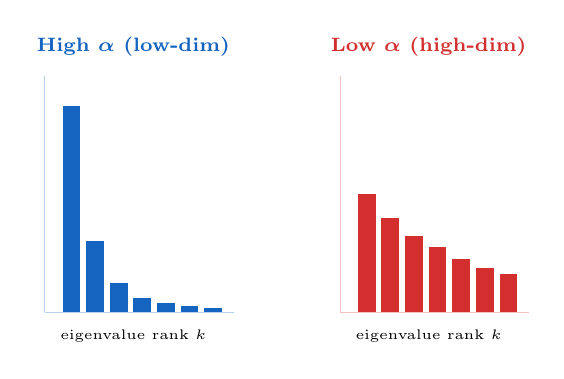
\begin{tikzpicture}[scale=0.75]
  % High alpha (low-dim)
  \node[font=\scriptsize\bfseries,dimlow] at (1.5,4.5) {High $\boldsymbol{\alpha}$ (low-dim)};
  \draw[dimlow!30,thin] (0,0) -- (0,4);
  \draw[dimlow!30,thin] (0,0) -- (3.2,0);
  \foreach \k/\h in {0.3/3.5, 0.7/1.2, 1.1/0.5, 1.5/0.25, 1.9/0.15, 2.3/0.1, 2.7/0.08} {
    \fill[dimlow] (\k,0) rectangle (\k+0.3,\h);
  }
  \node[font=\tiny] at (1.5,-0.4) {eigenvalue rank $k$};

  % Low alpha (high-dim)
  \node[font=\scriptsize\bfseries,dimhigh] at (6.5,4.5) {Low $\boldsymbol{\alpha}$ (high-dim)};
  \draw[dimhigh!30,thin] (5,0) -- (5,4);
  \draw[dimhigh!30,thin] (5,0) -- (8.2,0);
  \foreach \k/\h in {5.3/2.0, 5.7/1.6, 6.1/1.3, 6.5/1.1, 6.9/0.9, 7.3/0.75, 7.7/0.65} {
    \fill[dimhigh] (\k,0) rectangle (\k+0.3,\h);
  }
  \node[font=\tiny] at (6.5,-0.4) {eigenvalue rank $k$};
\end{tikzpicture}

\vspace{0.3em}
{\small Left: one eigenvalue dominates (steep decay). Right: many eigenvalues contribute (slow decay).}
\end{column}
\end{columns}
\end{frame}

%% --- SLIDE: Alpha tracks potent space ---
\begin{frame}{Metric dissociation tracks potent space size}

\begin{columns}[T]
\begin{column}{0.50\textwidth}
\textbf{The geometric dissociation index $\alpha$} anti-correlates with null-space fraction:

\vspace{0.6em}
\centering
{\scriptsize
\begin{tabular}{lcc}
\toprule
& $\rho$ & $p$ \\
\midrule
Nonlinear & $-0.86$ & $5 \times 10^{-22}$ \\
Linear (LDA) & $-0.68$ & $3 \times 10^{-11}$ \\
\bottomrule
\end{tabular}
}
\flushleft

\vspace{0.6em}
{\small Tools disagree most where \textbf{potent subspaces are largest}.}

\vspace{0.3em}
{\small But potent decoding accuracy does \emph{not} correlate with $\alpha$ ($\rho = -0.07$, $p = 0.57$). The signal is always there --- only its \textbf{relative size} varies.}
\end{column}

\begin{column}{0.47\textwidth}
\centering
\vspace{0.5em}
\textbf{Interpretation}

\vspace{0.5em}
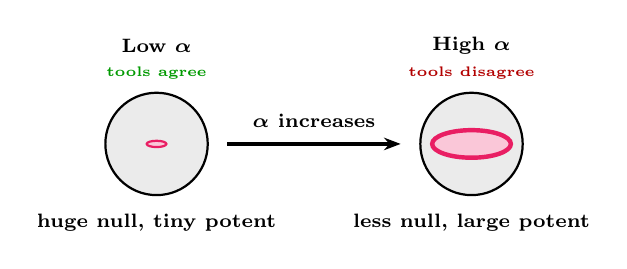
\begin{tikzpicture}[scale=0.5]
  \node[font=\scriptsize\bfseries] at (-1,4.5) {Low $\boldsymbol{\alpha}$};
  \node[font=\tiny\bfseries,green!60!black] at (-1,3.8) {tools agree};
  \fill[black!8] (-1,2) ellipse (1.3 and 1.3);
  \draw[black,thick] (-1,2) ellipse (1.3 and 1.3);
  \fill[choice!25] (-1,2) ellipse (0.25 and 0.08);
  \draw[choice,thick] (-1,2) ellipse (0.25 and 0.08);
  \node[font=\scriptsize\bfseries,black] at (-1,-0.0) {huge null, tiny potent};
  \node[font=\scriptsize\bfseries] at (7,4.5) {High $\boldsymbol{\alpha}$};
  \node[font=\tiny\bfseries,red!70!black] at (7,3.8) {tools disagree};
  \fill[black!8] (7,2) ellipse (1.3 and 1.3);
  \draw[black,thick] (7,2) ellipse (1.3 and 1.3);
  \fill[choice!25] (7,2) ellipse (1.0 and 0.35);
  \draw[choice,ultra thick] (7,2) ellipse (1.0 and 0.35);
  \node[font=\scriptsize\bfseries,black] at (7,-0.0) {less null, large potent};
  \draw[black,ultra thick,-{Stealth[length=6pt]}] (0.8,2) -- (5.2,2);
  \node[font=\scriptsize\bfseries] at (3,2.6) {$\boldsymbol{\alpha}$ increases};
\end{tikzpicture}

\vspace{0.3em}
{\small CKA is swamped by the null space. When the potent space grows, nonlinear tools catch it but linear tools still drown in null variance $\to$ dissociation.}
\end{column}
\end{columns}
\end{frame}

\section{5. Multi-task generalization}

%% --- SLIDE: Multi-task generalization ---
\begin{frame}{Multi-task generalization: subspaces for four variables}
\begin{columns}[T]
\begin{column}{0.48\textwidth}
\textbf{Beyond binary choice:}\\[0.3em]
{\small We trained subspaces for four task variables simultaneously: \textbf{choice}, \textbf{evidence strength}, \textbf{feedback}, and \textbf{stimulus side}.}

\vspace{0.5em}
{\small \textbf{Grassmannian distances between task subspaces:}}\\[0.3em]
{\scriptsize
\begin{tabular}{lccc}
\toprule
 & \textbf{Evidence} & \textbf{Feedback} & \textbf{Stim.\ side} \\
\midrule
\textbf{Choice} & large & large & \textcolor{fail}{small} \\
\textbf{Evidence} & --- & large & large \\
\textbf{Feedback} & & --- & large \\
\bottomrule
\end{tabular}
}

\vspace{0.5em}
{\small Choice and stimulus side share geometry (expected---they're correlated). Other pairs are separated: the learned subspaces don't collapse task variables into one direction.}
\end{column}
\begin{column}{0.50\textwidth}
\textbf{What this tests:}\\[0.2em]
{\small If the subspace method just found ``the interesting direction,'' all task subspaces would overlap. Instead:}
\vspace{0.2em}
{\small
\begin{itemize}\setlength\itemsep{1pt}
  \item 4 distinct subspaces per region
  \item Distances match expected task structure (choice $\approx$ stim.\ side $\neq$ feedback)
  \item Generalizes across 73 regions, 39 sessions
\end{itemize}
}

\vspace{0.3em}
{\small \textbf{Implication:} The geometric framework scales beyond binary choice. Each task variable occupies its own subspace, mirroring task structure.}
\end{column}
\end{columns}
\end{frame}

\section{6. Grassmannian dissimilarity}

%% --- SLIDE: Grassmannian dissimilarity matrices ---
\begin{frame}{Grassmannian dissimilarity matrices}
\begin{columns}[T]
\begin{column}{0.50\textwidth}
\textbf{Method:} Compute $73 \times 73$ pairwise Grassmannian distances between subspaces found by LDA (linear), a nonlinear decoder, and CKA.

\vspace{0.5em}
\textbf{Result:} Linear and nonlinear dissimilarity matrices are nearly identical ($\rho = 0.97$). Both \emph{anti-correlate} with CKA.

\vspace{0.5em}
\textbf{Interpretation:} Linear and nonlinear methods agree on \emph{which regions are similar}---they disagree on \emph{what matters within each region}. CKA sees a different structure entirely.
\end{column}

\begin{column}{0.47\textwidth}
\vspace{0.5em}
{\small
\begin{tabular}{lc}
\toprule
\textbf{Comparison} & \textbf{$\rho$} \\
\midrule
Linear GDM vs Nonlinear GDM & 0.97 \\
Linear GDM vs CKA & $< 0$ \\
Nonlinear GDM vs CKA & $< 0$ \\
\bottomrule
\end{tabular}
}

\vspace{0.8em}
{\small This is a ``neural taskonomy'': the functional hierarchy of brain regions, measured through the geometry of their choice subspaces rather than through their activity patterns.}
\end{column}
\end{columns}
\end{frame}

\section{7. Cross-dataset replication (IBL)}

%% --- SLIDE: IBL replication headline ---
\begin{frame}{The CKA--Procrustes dissociation replicates in an independent dataset}
\vspace{-0.5em}
\begin{center}
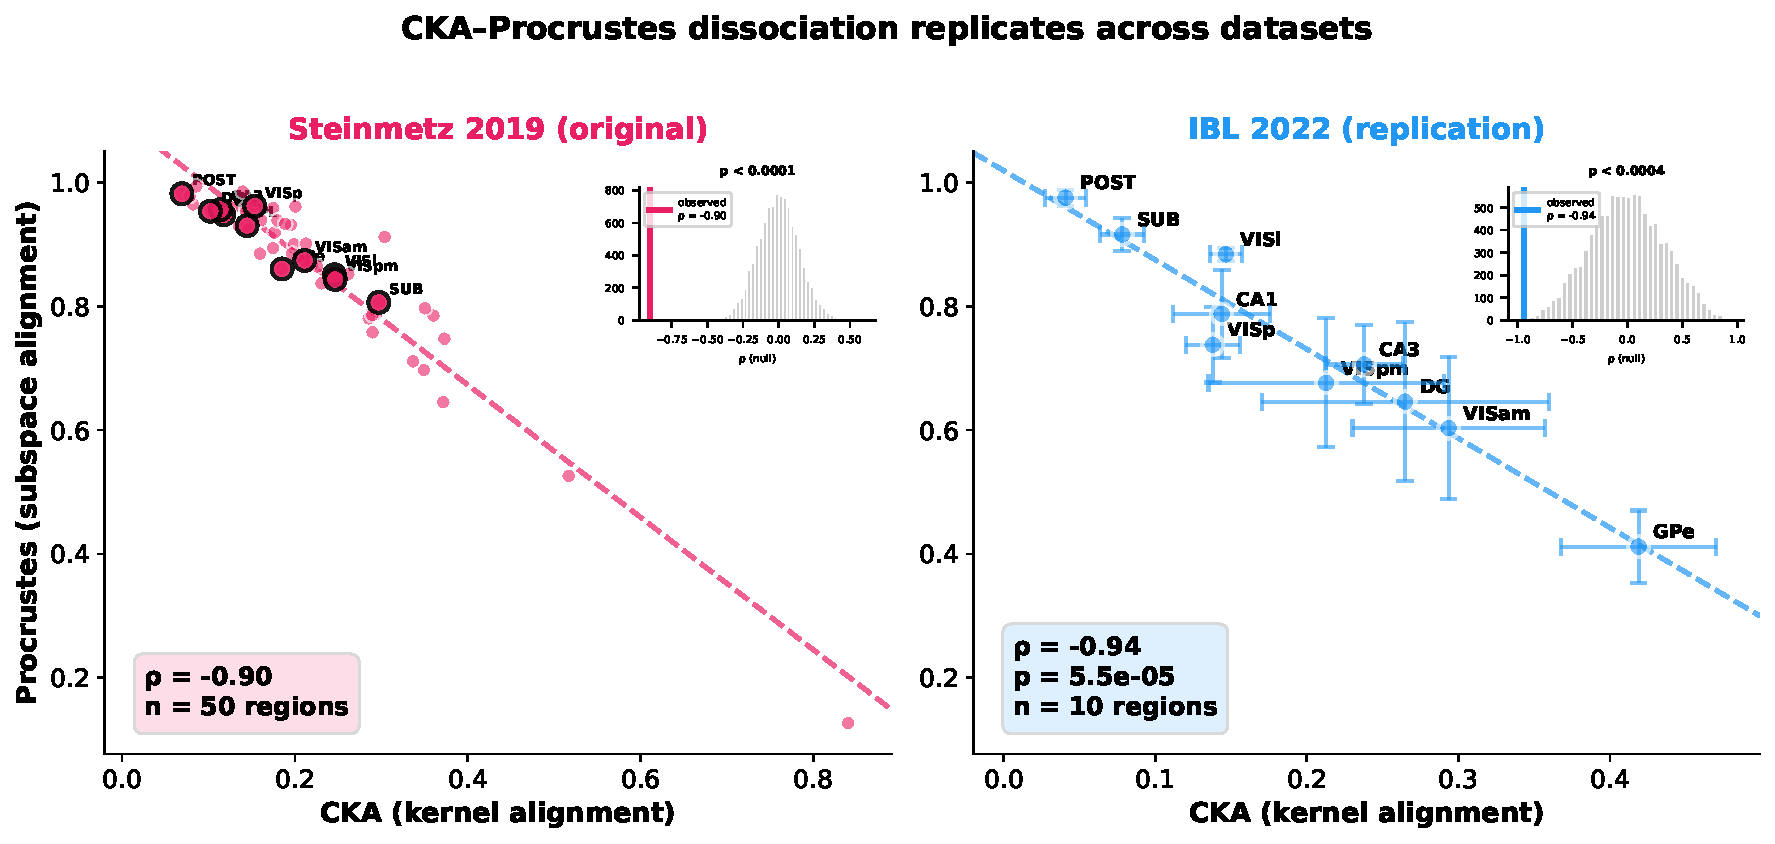
\includegraphics[width=0.95\textwidth]{cross_dataset_anticorrelation.pdf}
\end{center}

\vspace{-0.5em}
{\scriptsize \textbf{Left:} Steinmetz 2019 (50 regions, $\rho = -0.90$). \textbf{Right:} IBL 2022 (10 regions, $\rho = -0.94$, $p = 5.5 \times 10^{-5}$). Dissociation is \textit{stronger} in the replication.}
\end{frame}

%% --- SLIDE: IBL per-region CKA vs Procrustes bars ---
\begin{frame}{IBL regions show the same CKA--Procrustes inversion}
\begin{columns}[T]
\begin{column}{0.52\textwidth}
\vspace{-0.3em}
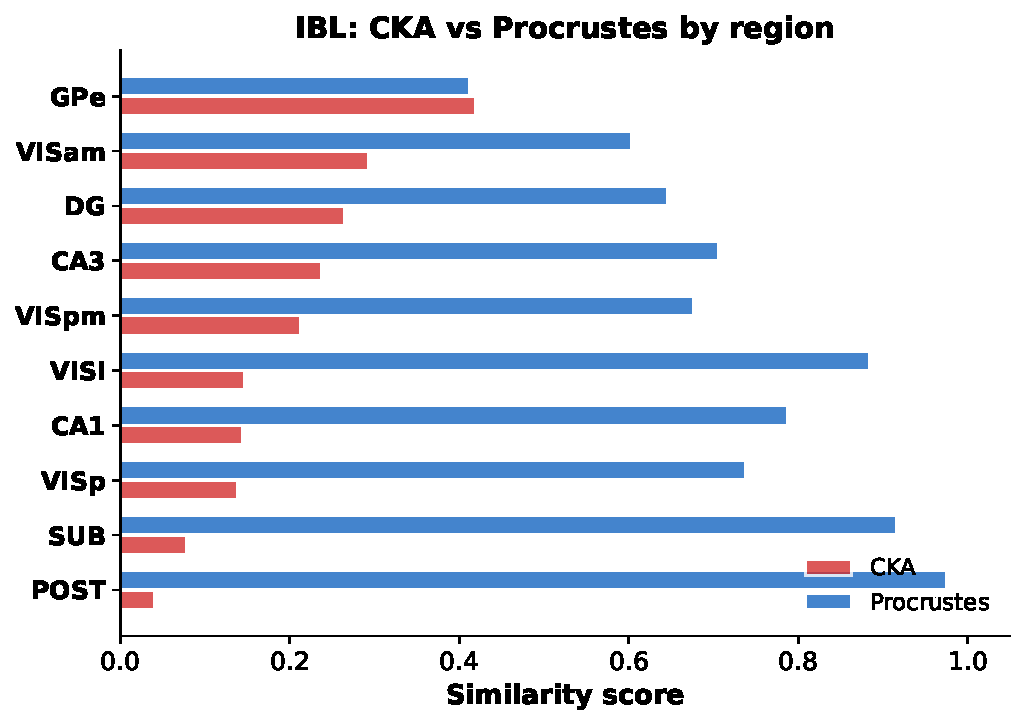
\includegraphics[width=\textwidth]{ibl_cka_proc_bars.pdf}
\end{column}
\begin{column}{0.46\textwidth}
\vspace{0.5em}
\textbf{Key observations:}
\begin{itemize}\setlength\itemsep{0.15em}
  \item POST, SUB: extreme Procrustes-dominant (low-dim, strong geometric alignment)
  \item GPe: balanced transition point (CKA $\approx$ Procrustes)
  \item Every region shows the inversion
\end{itemize}

\vspace{0.3em}
{\scriptsize 10 regions with $\geq 3$ IBL sessions. CKA and Procrustes computed on session-pair similarity matrices.}
\end{column}
\end{columns}
\end{frame}

%% --- SLIDE: Classification transfer ---
\begin{frame}{Region type classifications partially transfer}
\begin{columns}[T]
\begin{column}{0.55\textwidth}
\vspace{-0.3em}
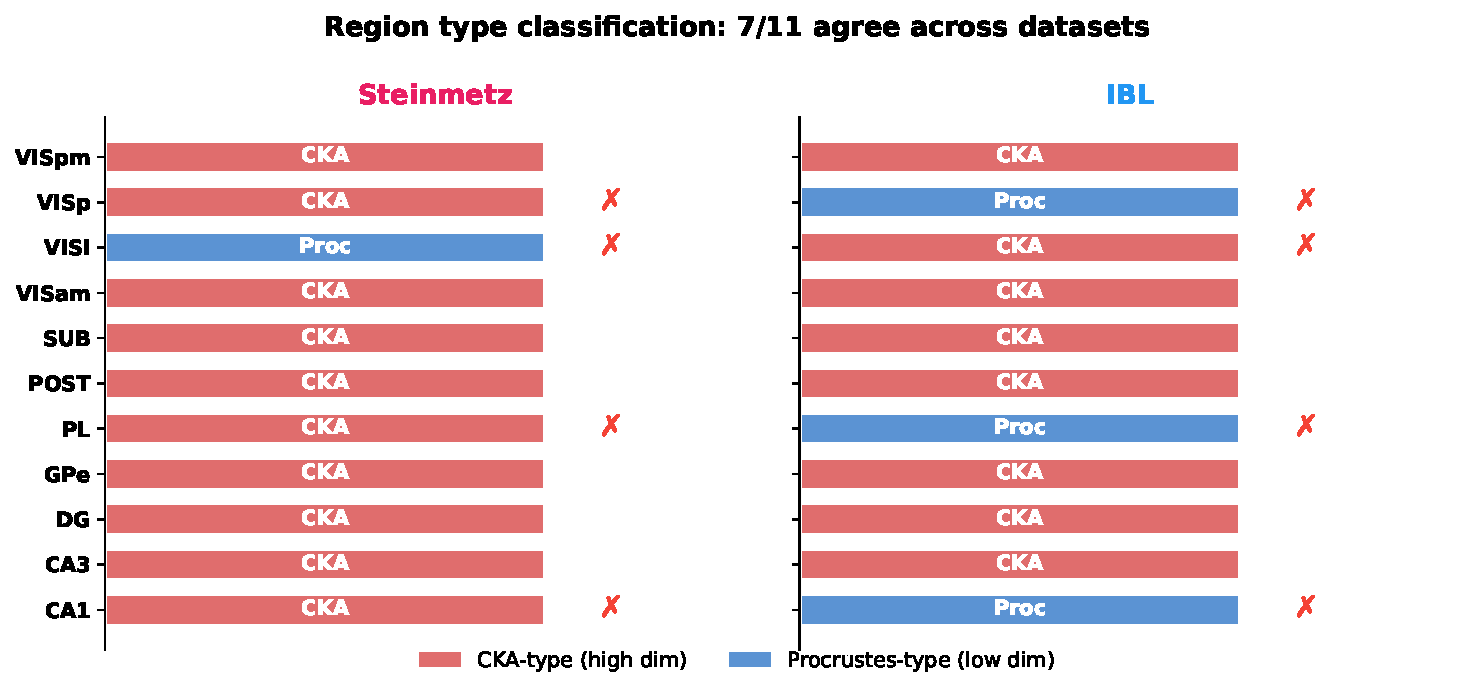
\includegraphics[width=\textwidth]{cross_dataset_classification.pdf}
\end{column}
\begin{column}{0.43\textwidth}
\vspace{0.3em}
\begin{itemize}\setlength\itemsep{0.15em}
  \item 7/11 regions keep the same type
  \item Mismatches (CA1, PL, VISl, VISp) are near the $\alpha = 1.5$ threshold
  \item The \textit{continuous} correlation ($\rho = -0.94$) replicates; the binary split is noisier
\end{itemize}

\vspace{0.3em}
{\scriptsize Threshold-based classification is sensitive to small $\alpha$ shifts. The continuous relationship is robust.}
\end{column}
\end{columns}
\end{frame}

%% --- SLIDE: Alpha does not transfer ---
\begin{frame}{Power-law exponent does not transfer, but the dissociation does}
\begin{columns}[T]
\begin{column}{0.55\textwidth}
\vspace{-0.3em}
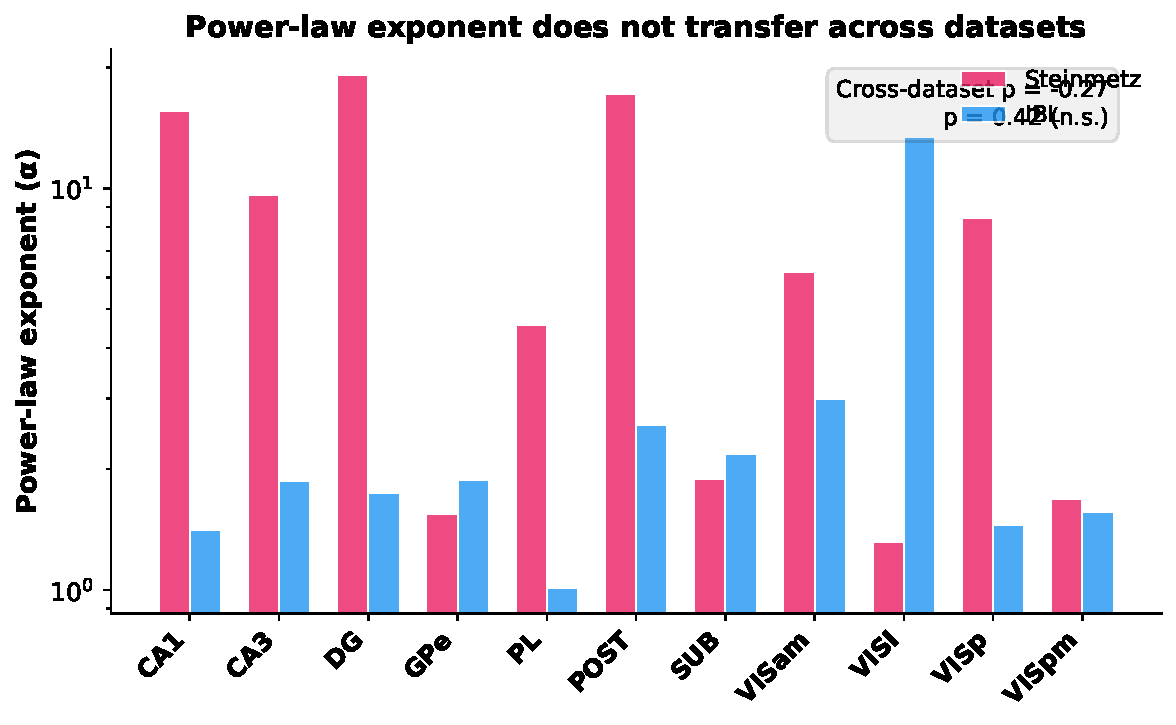
\includegraphics[width=\textwidth]{cross_dataset_alpha.pdf}
\end{column}
\begin{column}{0.43\textwidth}
\vspace{0.3em}
\textbf{What transfers:}
\begin{itemize}\setlength\itemsep{0.05em}
  \item CKA--Procrustes anti-correlation ($\rho = -0.94$)
  \item Relative region ordering
\end{itemize}

\vspace{0.3em}
\textbf{What does not:}
\begin{itemize}\setlength\itemsep{0.05em}
  \item Absolute $\alpha$ values ($\rho = -0.27$, n.s.)
  \item Sensitive to recording quality, spike sorting, neuron yield
\end{itemize}

\vspace{0.3em}
{\scriptsize The \textit{geometric relationship} between metrics is a property of population structure, not of any particular recording pipeline.}
\end{column}
\end{columns}
\end{frame}

%% --- SLIDE: IBL replication summary ---
\begin{frame}{Cross-dataset replication: what we learned}
\vspace{-0.2em}
\begin{columns}[T]
\begin{column}{0.48\textwidth}
\textbf{\textcolor{pass}{Replicates:}}
\begin{itemize}\setlength\itemsep{0.15em}
  \item CKA--Procrustes anti-correlation: $\rho = -0.94$ in IBL vs $-0.90$ in Steinmetz
  \item Every IBL region shows the CKA--Procrustes inversion
  \item 7/11 regions keep their type classification
  \item Matched regions occupy similar positions in CKA--Procrustes space
\end{itemize}
\end{column}
\begin{column}{0.48\textwidth}
\textbf{\textcolor{fail}{Does not replicate:}}
\begin{itemize}\setlength\itemsep{0.15em}
  \item Absolute power-law exponent ($\rho = -0.27$, n.s.)
  \item Binary type classification at the threshold boundary (4 mismatches)
\end{itemize}

\vspace{0.5em}
\textbf{Interpretation:}\\[0.2em]
{\small The geometric \textit{relationship} between metrics is a property of neural populations, not of recording pipelines. The absolute metric values are not.}
\end{column}
\end{columns}
\end{frame}

\section{Conclusions}

%% --- SLIDE: Limitations ---
\begin{frame}{Project limitations}
\begin{columns}[T]
\begin{column}{0.5\textwidth}
\textbf{Hard limits (sample size):}
\begin{itemize}
  \item \textbf{Two datasets} (Steinmetz 2019 + IBL 2022), but both are mouse Neuropixels
  \item \textbf{10 mice} (Steinmetz): too few to quantify individual differences
  \item \textbf{Binary choice only}---does metric dissociation generalize to richer tasks?
\end{itemize}
\end{column}
\begin{column}{0.48\textwidth}
\textbf{What comes next:}
\begin{itemize}
  \item \textbf{More IBL regions}: 19 searched, 11 yielded data---expand with looser neuron thresholds
  \item \textbf{Richer tasks}: multi-variable, continuous, naturalistic---is the Grassmannian structure task-general?
  \item \textbf{Other species}: do primate recordings show the same potent/null geometry?
\end{itemize}
\end{column}
\end{columns}
\end{frame}

%% --- SLIDE: Summary ---
\begin{frame}{Summary}
\begin{columns}[T]
\begin{column}{0.5\textwidth}
\textbf{Core geometric findings:}
\begin{enumerate}
  \item CKA and Procrustes anti-correlate ($\rho = -0.90$, replicates at $-0.94$ in IBL); dimensionality explains why
  \item Variance structure is universal ($0.94$); neural content is not ($0.09$)
  \item Geometry predicts decoder performance ($r = -0.51$) and dimensionality predicts metric dissociation ($\rho = -0.48$)
\end{enumerate}
\end{column}
\begin{column}{0.48\textwidth}
\textbf{Deeper geometric structure:}
\begin{enumerate}
  \setcounter{enumi}{3}
  \item Potent/null decomposition explains metric dissociation ($\rho = -0.86$); null space fraction is the key mediator
  \item Four task variables occupy distinct subspaces on the Grassmannian, mirroring task structure
  \item Grassmannian dissimilarity reveals a neural taskonomy where linear and nonlinear methods agree ($\rho = 0.97$) but both anti-correlate with CKA
\end{enumerate}
\end{column}
\end{columns}

\vspace{0.5em}
{\small \textbf{Takeaway:} Dimensionality mediates tool disagreement, potent/null structure explains why, Grassmannian geometry captures functional organization, and the dissociation replicates across independent datasets.}
\end{frame}

%% --- SLIDE: Conclusion ---
\begin{frame}{Conclusion}

\begin{center}
\vspace{0.5em}
{\Large Neural geometry is \textbf{not metric-neutral}.}

\vspace{0.6em}

{\Large The tool you choose determines what you find,}

\vspace{0.2em}

{\Large and \textbf{dimensionality} tells you which tool to trust.}
\end{center}
\end{frame}

%% --- SLIDE: Thank you ---
\begin{frame}{Thank you}

\textbf{Paper:} TBD

\vspace{0.3em}
\textbf{Repository:} \href{https://github.com/elliottower/causal-geometry-neuro}{\texttt{github.com/elliottower/causal-geometry-neuro}}

\vspace{0.3em}
\textbf{Contact:} \texttt{elliot@elliottower.com}

\vspace{0.3em}
{\small
\textbf{Data sources:}
\begin{itemize}\setlength\itemsep{0pt}
  \item \href{https://doi.org/10.1038/s41586-019-1787-x}{Steinmetz et al.\ 2019} --- 73 brain regions, 39 sessions, 10 mice, ${\sim}30{,}000$ neurons (Neuropixels)
  \item \href{https://int-brain-lab.github.io/}{IBL Brain-Wide Map 2022} --- 11 matched regions, 139 mice, 12 labs (replication dataset)
  \item \href{https://connectivity.brain-map.org/}{Allen Mouse Brain Atlas} --- structural connectivity + CCF atlas for region mapping
\end{itemize}

\textbf{Experiments:} Modal A10G GPUs
}
\end{frame}

%% --- SLIDE: References ---
\begin{frame}{References (1/2)}
\vspace{-0.3em}
{\scriptsize
\begin{itemize}\setlength\itemsep{0pt}
  \item Arbour et al.\ (2016). \href{https://www.auai.org/uai2016/proceedings/papers/217.pdf}{Inferring causal direction from relational data.} UAI.
  \item Craver (2007). \href{https://doi.org/10.1093/acprof:oso/9780199299317.001.0001}{Explaining the Brain.} Oxford University Press.
  \item Esmaeili et al.\ (2019). \href{https://proceedings.mlr.press/v89/esmaeili19a}{Structured disentangled representations.} AISTATS.
  \item Gallego et al.\ (2017). \href{https://doi.org/10.1038/nn.4510}{Neural manifolds for the control of movement.} \textit{Neuron}.
  \item Kaufman et al.\ (2014). \href{https://doi.org/10.1038/nn.3643}{Cortical activity in the null space.} \textit{Nature Neuroscience}.
  \item Maier et al.\ (2013). \href{https://arxiv.org/abs/1309.6843}{A sound and complete algorithm for learning causal models from relational data.} UAI.
  \item Mayo (2018). \href{https://doi.org/10.1017/9781107286184}{Statistical Inference as Severe Testing.} Cambridge University Press.
\end{itemize}
}
\end{frame}

\begin{frame}{References (2/2)}
\vspace{-0.3em}
{\scriptsize
\begin{itemize}\setlength\itemsep{0pt}
  \item Pearl \& Bareinboim (2011). \href{https://arxiv.org/abs/1203.3519}{Transportability of causal and statistical relations.} AAAI.
  \item Shallice (1988). \href{https://doi.org/10.1017/CBO9780511526817}{From Neuropsychology to Mental Structure.} Cambridge University Press.
  \item Steinmetz et al.\ (2019). \href{https://doi.org/10.1038/s41586-019-1787-x}{Distributed coding of choice, action and engagement across the mouse brain.} \textit{Nature}.
  \item Sussillo \& Barak (2013). \href{https://doi.org/10.1162/NECO_a_00409}{Opening the black box: low-dimensional dynamics in high-dimensional recurrent neural networks.} \textit{Neural Computation}.
  \item Vyas et al.\ (2020). \href{https://doi.org/10.1146/annurev-neuro-092619-094115}{Computation through neural population dynamics.} \textit{Annual Review of Neuroscience}.
  \item Woodward (2003). \href{https://doi.org/10.1093/0195155270.001.0001}{Making Things Happen.} Oxford University Press.
\end{itemize}
}
\end{frame}

\end{document}
